\documentclass[iop]{emulateapj}
\usepackage{graphicx}
\usepackage{amssymb}
\usepackage{epstopdf}
\usepackage{amsmath}
\usepackage[breaklinks]{hyperref}
\usepackage{ulem}

\DeclareGraphicsRule{.tif}{png}{.png}{`convert #1 `dirname #1`/`basename #1 .tif`.png}
\citestyle{aa}

%\date{}                                           % Activate to display a given date or no date

%---------------------------- Physical Quantities ------------------------------------%
\newcommand{\kms}{\ensuremath{\rm km\,s^{-1}}}
\newcommand{\ms}{\ensuremath{\rm m\,s^{-1}}}
\newcommand{\mse}{\ensuremath{\rm m\,s^{-1}}}
\newcommand{\gcmc}{\ensuremath{\rm g\,cm^{-3}}}
\newcommand{\gcc}{\gcmc}
\newcommand{\fluxunit}{\ensuremath{\rm erg\,s^{-1}\,cm^{-2}}}
\newcommand{\rhk}{\ensuremath{R^{\prime}_{\rm HK}}}	% Activity index R'_HK
\newcommand{\logrhk}{\ensuremath{\log\rhk}}		% log of R'_HK

\newcommand{\teff}{\ensuremath{T_{\rm eff}}}
\newcommand{\logg}{\ensuremath{\log{g}}}
\newcommand{\vsini}{\ensuremath{v \sin{i}}}
\newcommand{\feh}{[Fe/H]}
\newcommand{\logl}{\ensuremath{\log{L}}}

\newcommand{\rsun}{\ensuremath{R_\sun}}
\newcommand{\msun}{\ensuremath{M_\sun}}
\newcommand{\lsun}{\ensuremath{L_\sun}}

\newcommand{\rstar}{\ensuremath{R_\star}}
\newcommand{\mstar}{\ensuremath{M_\star}}
\newcommand{\loggstar}{\ensuremath{\logg_\star}}
\newcommand{\lstar}{\ensuremath{L_\star}}
\newcommand{\astar}{\ensuremath{a_\star}}
\newcommand{\loglstar}{\ensuremath{\log{L_\star}}}
\newcommand{\rhostar}{\ensuremath{\rho_\star}}

\newcommand{\rpl}{\ensuremath{R_{\rm P}}}
\newcommand{\mpl}{\ensuremath{M_{\rm P}}}
\newcommand{\lpl}{\ensuremath{L_{\rm P}}}
\newcommand{\rhopl}{\ensuremath{\rho_{\rm P}}}
\newcommand{\loggpl}{\ensuremath{\logg_{\rm P}}}
\newcommand{\teq}{\ensuremath{T_{\rm eq}}}

\newcommand{\rjup}{\ensuremath{R_{\rm J}}}
\newcommand{\mjup}{\ensuremath{M_{\rm J}}}
\newcommand{\rhojup}{\ensuremath{\rho_{\rm J}}}
\newcommand{\rearth}{\ensuremath{R_\earth}}
\newcommand{\mearth}{\ensuremath{M_\earth}}
\newcommand{\fearth}{\ensuremath{F_\earth}}

\newcommand{\msini}{\ensuremath{m \sin{i}}}
\newcommand{\mplsini}{\ensuremath{\mpl\sin{i}}}

\newcommand{\npl}{243~} % The number of exoplanets used to determine the MRF relation
\newcommand{\nhires}{42~} % The number of transiting planets in the HIRES paper
\newcommand{\nlm}{59~}
\newcommand{\rspecial}{4 \rearth}
\newcommand{\chisquared}{2.2~}
\newcommand{\chiquad}{6.5~}
\newcommand{\rms}{3.8 \mearth}

\begin{document}
\title{A Relation between Mass and Radius for 59 Exoplanets Smaller than 4 Earth Radii}
\author{Lauren~M.~Weiss$^{1,\dagger}$ \& Geoffrey~W.~Marcy$^1$}
\affil{$^1$B-20 Hearst Field Annex, Astronomy Department, University of California, Berkeley, CA 94720}
\altaffiltext{$\dagger$}{\small Supported by the NSF Graduate Student Fellowship, Grant DGE 1106400.}

\begin{abstract}
We study the masses and radii of 59 exoplanets smaller than 4\rearth.  We find a linear relation $\mpl/\mearth = 0.21 + 2.78\rpl/\rearth$.  The RMS of planet masses to the linear fit is \rms, and our best fit has reduced $\chi^2=\chisquared$, indicating a large diversity in planet compositions below 4\rearth.  The exoplanets in our sample have orbital periods between 0 and 100 days.  \citet{WL2013} find $\mpl = 3\rpl$ in 22 pairs of planets exhibiting transit timing variations, of which only 10 planets overlap with our sample.  The linear mass-radius relation translates to a decrease in planet density with increasing radius ($\mpl \propto \rhopl^{-2}$).  We find that exoplanets have densities comparable to that of Earth at 1.6\rearth; exoplanets smaller than 1.6\rearth\ are typically denser than Earth, indicating likely rocky compositions, whereas exoplanets larger than 1.6\rearth\ are typically less dense than Earth, indicating a significant fraction of H/He or water in their compositions.
\end{abstract}

\section{Introduction}
%\subsection{}

The Kepler Mission has found an abundance of planets with  $R < 4\rearth$ \citep{Batalha2013, Burke2013}.  However, in many systems, it is difficult to measure the masses of such small planets because the gravitational acceleration these planets induce on their host stars or neighboring planets is too small to detect with current telescopes and instruments.  Obtaining measurements of the masses of these planets and characterizing their compositions is vital to understanding the formation and evolution of these planets.

Many scientists have explored the relation between planet mass and radius in the Solar system and beyond as a means for understanding exoplanet compositions \citep{Lissauer2011, Enoch2012, Kane2012, Seager2007}.  \citet{Weiss2013} have shown that for planets between a few and 150 of Earth masses, we can predict the radius of a planet from its mass and incident stellar flux.  However, below 4\rearth, the large apparent scatter in planet mass impedes accurate predictions of planet mass.  At 2\rearth, planets are observed to span a decade in density, from less dense than water to densities suggesting a solid iron composition.  One way to probe the scatter in planet mass is to attempt to measure the masses of more small planets.  

\section{Selecting Exoplanets with Measured Mass and Radius}
Although uncertainties in the mass measurements for individual planets might be of order the planet mass, weak constraints on the masses of many small planets allow us to study the statistical distribution of planet masses for small planets.  \citet{Marcy2013} measured the masses of 42 small, transiting planets.  The planets were selected for their small size, and not based on predictions of their masses.  Therefore, these 42 new transiting planets offer an unbiased survey of the masses of small planets.  In this paper, we examine the relation between exoplanet mass and radius for the 40 exoplanets smaller than 4\rearth\ from \citet{Marcy2013}, plus 19 exoplanets smaller than 4\rearth\ from the literature, for a total of 59 exoplanets.  We also investigate how orbital parameters and stellar physical properties, including the planet's orbital period and semi-major axis, the incident flux from the star on the planet, and the stellar mass, radius, temperature, metallicity, and rotation, correlate with the residuals of the mass-radius relation.

\subsection{Including Mass Non-Detections for Statistical Soundness}
At a given radius, if we only include detections exceeding a certain confidence, we will preferentially include high-mass planets and will fail to include the low-mass planets that have comparable errors.  This is especially true for small planets, for which the planet-induced RV signal ($\sim1\ms$) can be small compared to the noise from stellar activity ($\sim5\ms$).  Although there is no physical reason that the stellar activity should phase with the orbit of a planet, random statistical fluctuations in the RVs can produce RVs that are high when they should be high, and low when they should be low, or the converse (RVs that are low when they should be high, and high when they should be low).  Because RVs from stellar activity that phase with the expected planet signal will result in an over-estimate of planet mass, we must also include the RVs that are anti-phased with the expected planet signal.  When \citet{Marcy2013} phase the RV measurements to the transit-determined planet ephemeris, they allow  a negative semi-amplitude in the Keplerian fit to the RVs that results in a ``negative" planet mass determination.  Classically, these planets are considered non-detections, but we include them in the mass-radius relation to avoid statistical bias toward large planet masses at a given radius.  Since there is no bias toward large or small planet masses in our sample, we can take the weighted mean mass of planets of a given radius and get a value representative of the planet population.

\section{The Mass-Radius Relation for 59 Small Exoplanets}
On average, exoplanet mass increases with increasing radius, indicating an underlying correlation in the individual exoplanet masses and radii.  The individual measurements of planet mass and radius are shown in Figure \ref{fig:rm_4} and listed in Table \ref{tab:mrf}.  In Figure \ref{fig:rm_4}, we show the weighted mean exoplanet mass in bins of width 1 \rearth\ to highlight the correlation between planet mass and radius.

We calculate the probability that mass and radius are uncorrelated for planets smaller than 4\rearth.  We calculate the correlation coefficient (Pearson R test) $r=0.61$.  In our sample of 59 exoplanets, the probability that these data are uncorrelated given $r = 0.61$ is $1.3 \times 10^{-6}$.  Thus, the masses and radii of planets between the sizes of Earth and Neptune are correlated.

The individual masses and radii shown in Figure \ref{fig:rm_4} suggest that exoplanet masses can be fit with a line.  We verify this with a traditional power-law fit and obtain $\mpl \propto \rpl$ as the best result.

The weighted linear fit to the data for $\rpl < \rspecial$ is:
\begin{equation}
\mpl/\mearth = -0.7 +     3.0~\rpl/\rearth
\label{eqn:mr_relation}
\end{equation}
There are 59 exoplanets in this sample.  The reduced $\chi^2=\chisquared$, and the RMS $=\rms$.  The standard errors for the weighted linear fit are $slope = 3.0 \pm 0.6$, $intercept=-0.7\pm1.2$.

To illustrate how this population of exoplanets compares to our Solar System, we indicate the Solar System planets in Figure \ref{fig:rm_4}.  A quadratic fit to the exoplanet population happens to line up with the Solar System planets, but has a reduced $\chi^2$ that is twice as large as the linear fit to the exoplanets.  Since most of the exoplanets in this sample have $P < 50$ days, we do not expect them to behave the same way as Uranus and Neptune, which have orbital periods of tens of thousands of days.  Therefore, the hefty masses of Uranus and Neptune compared to planets of similar size that are closer to their stars is not unreasonable.

\section{Discussion}
	
\subsection{Interpretation of the Mass-Radius Relation}
The correlation between exoplanet mass and radius for $\rpl < 4 \rearth$ indicates that Earth-size planets are less massive than Neptune-size planets.

The large reduced $\chi^2$ values for the linear and quadratic mass-radius relations indicate that these relations are not sufficient models to explain the variation in planet mass at a given radius.  A diversity of planet compositions, perhaps elucidated by correlation between the residuals and some other parameter, is required to explain the large scatter in planet mass.

The linear relation between planet mass and radius results in $\rhopl \propto \rpl^{-2}$, indicating that planet density decreases strongly as mass and radius increase (see Figure \ref{fig:rm_4}).  This can be attributed to an increasing fraction of volatiles with increasing planet mass.

The large fractional mass errors for $\rpl < 1 \rearth$ result in huge density errors.  Although the planets smaller than 1\rearth\ do not have mass detections better than 2$\sigma$, their ensemble provides weak constraints on the expected mass of planets smaller than Earth.  For instance, none of the planets smaller than Earth has a mass larger than 10\mearth, and most have $\mpl < 5\mearth$.  Because we allow for negative planet masses in this regime, the weighted mean mass for planets between 0 and 1 \rearth\ should not be statistically biased.

The reader might wonder if removing low-significance mass determinations would improve the robustness of the fit.  In Figure \ref{fig:rm_4_1sig}, we use only the 42 exoplanets that have mass determinations of $1\sigma$ and better, which excludes most of the planets in the 0-1 \rearth\ bin.  The linear trend is still apparent, and the slope and intercept are similar to those in the less discriminating fit.  However, we can see bias in this fit.  The surviving small planets have larger masses than the discarded planets did, and so the intercept of the fit is higher, and the slope is shallower.

Previous work, including \citet{Lissauer2011} and \citet{Weiss2013}, suggest that the mass-radius relation is more like $\mpl \propto \rpl^2$ for small exoplanets.  However, these studies include Saturn or Saturn-like planets at the high-mass end of their populations.  Such planets are better described as part of the giant planet population and are not useful in determining an empirical mass-radius relation for small exoplanets.  Excluding Saturn-like planets gives a linear mass-radius relation for small planets.

In a study of planets with $\mpl < 20\mearth$, \citet{WL2013} found $\mpl/\mearth = 3 \rpl/\rearth$ in a sample of 22 pairs of planets that exhibited strong anti-correlated transit timing variations (TTVs).  Our independent assessment of 59 planets, 49 of which are not analyzed in \citet{WL2013}, agrees with this result.

\citet{WL2013} noted that a linear relation between planet mass and radius is dimensionally consistent with a constant escape velocity from the planet (i.e. $v_{\mathrm{esc}}^2 \sim \mpl/\rpl$).  The linear mass-radius relation might result from photo-evaporation of the atmospheres of small planets near their stars.

\subsection{Interpretation of Planet Compositions}
For detailed models of the compositions of the 42 new transiting planets presented in \citet{Marcy2013} and analyzed here, see \citet{Rogers2013}.  Here, we consider the statistical properties of planet densities.

The densities of exoplanets with $\rpl < \rspecial$ and the densities binned by 1 \rearth\ are shown in Figure \ref{fig:rm_4}.  These data show that smaller planets have higher densities, and planets have an Earth-density at 1.6 \rearth.  Planets smaller than 1.6 \rearth\ tend to be denser than Earth, whereas planets larger than 1.6 \rearth\ tend to be less dense than Earth.  However, since rock and other materials are compressible, planets that are as dense as Earth but have larger radii are not necessarily solid rock; they need some lighter materials, such as water or a H/He envelope, to achieve the density of Earth.

\subsection{Absence of Correlations to Planet Mass Residuals}
We examine the possibility that the residuals to the mass-radius relation correlate with some other parameters.  We consider how the residual mass (exoplanet mass minus predicted mass), or, where more intuitive, residual radius (exoplanet radius minus predicted radius given the mass) correlates with various orbital properties and physical properties of the star.  The quantities we consider are: planet orbital period, planet semi-major axis, the incident flux from the star on the planet, stellar mass, stellar radius, stellar temperature, stellar metallicity, stellar age, .  The residual mass does not correlate with any of these properties; the highest Pearson-R coefficient is $0.1$.  While we cannot rule out correlation between the mass residuals and other orbital and physical properties, we do not find evidence for any correlation to the residuals.

\subsubsection{A Weak Correlation between Residual Planet Mass and Stellar Metallicity}
The stellar metallicities of the stars in our sample are determined by spectroscopy and/or asteroseismology, yielding values accurate to 0.1 dex.  We find a correlation between residual planet mass and stellar metallicity for planets smaller than 4\rearth.  The Pearson R-value of the correlation is 0.25, resulting in a probability of 5.8\% that the residual planet mass and stellar metallicity are not correlated.  In other words, we find a correlation between residual planet mass and metallicity with $2\sigma$ confidence in exoplanets smaller than 4\rearth.  In Figure \ref{fig:resids}, we plot residual planet mass and against stellar metallicity for the planets in our sample.

\citet{Buchhave2012} note that planets smaller than 4\rearth\ form around stars with a large range of metallicities.  Their study includes 226 Kepler exoplanet candidates smaller than 4\rearth, for which they obtained spectroscopic measurements of [m/H] in the host stars.  Our work uses [Fe/H] as a metallicity indicator, and we are only considering validated exoplanets.  Although \citet{Buchhave2012} find no relation between exoplanet occurrence and host star metallicity for $\rpl < 4\rearth$, they do not comment on the relation between exoplanet size and host star metallicity for small planets.  Therefore, our finding that planet mass correlates with stellar metallicity for $\rpl < 4\rearth$ does not contradict their result.


\section{Conclusions}
For exoplanets with $\rpl < \rspecial$ and $P < 100$ days, planet radius correlates with planet mass with linear scaling, indicating that larger planets have substantially more volatiles than smaller planets.  This relation is also different than the quadratic relation observed for the Solar System planets (excluding Jupiter).  Uranus and Neptune are more massive than the exoplanets of their size in this sample, and they are also at much larger orbital distances than any of the exoplanets in our sample.  A study of exoplanets of 3-4 \rearth\ with orbital periods of dozens of years would better contextualize the mass and radius of Uranus and Neptune.

One reason Uranus and Neptune might be more massive than closer-in planets of the same size is that incident stellar flux might photo evaporate the atmospheres of closer-in counterparts, causing mass loss.  The correlations between planet size and incident flux from the star for both large and small planets, and the absence of hot Neptunes, indicate that incident stellar flux of more than 100 times what Earth receives might play a key role in sculpting close-in planets.

%% The values (usually only l,r and c) in the last part of
%% \begin{deluxetable}{} command tell LaTeX how many columns
%% there are and how to align them.
\begin{deluxetable*}{lllllll}

%% Keep a portrait orientation


%% Over-ride the default font size
%% Use 10pt
\tabletypesize{\tiny}

\tablewidth{0pt} %to over-ride the default table width.
%% If you are unhappy with the default look at the end of the
%% *.log file to see what the default was set at before adjusting
%% this value.

%% This is the title of the table.
\tablecaption{Exoplanets with Mass Upper Limits and $\rpl < \rspecial$}
%% This command over-rides LaTeX's natural table count
%% and replaces it with this number.  LaTeX will increment 
%% all other tables after this table based on this number
\tablenum{1}
\label{tab:mrf}

%% The \tablehead gives provides the column headers.  It
%% is currently set up so that the column labels are on the
%% top line and the units surrounded by ()s are in the 
%% bottom line.  You may add more header information by writing
%% another line between these lines. For each column that requries
%% extra information be sure to include a \colhead{text} command
%% and remember to end any extra lines with \\ and include the 
%% correct number of &s.
\tablehead{\colhead{Name} & \colhead{Per} & \colhead{Mass} & \colhead{Radius} & \colhead{Flux} & \colhead{First Ref.} & \colhead{Mass Ref.} \\ 
\colhead{} & \colhead{(d)} & \colhead{($\mearth$)} & \colhead{($\rearth$)} & \colhead{($\fearth$)} & \colhead{} & \colhead{} } 

%% All data must appear between the \startdata and \enddata commands
\startdata
            55 Cnc e &      0.737 &       8.38$\pm$0.39       &       2.21$\pm$0.15       &   2439.690 &                     \citet{McArthur2004} &                         \citet{Endl2012}\\ 
           CoRoT-7 b &      0.854 &       5.02$\pm$0.86       &       1.68$\pm$0.09       &   1779.433 &             \citet{Queloz2009,Leger2009} &                       \citet{Queloz2009}\\ 
           GJ 1214 b &      1.580 &       6.26$\pm$0.91       &       2.80$\pm$0.24       &     16.631 &                  \citet{Charbonneau2009} &                       \citet{Carter2011}\\ 
          HD 97658 b &      9.491 &       7.87$\pm$0.73       &       2.34$\pm$0.16       &     48.106 &                       \citet{Howard2011} &                     \citet{Dragomir2013}\\ 
         Kepler-10 b &      0.837 &       4.54$\pm$1.25       &       1.42$\pm$0.03       &   3572.048 &                      \citet{Batalha2011} &                      \citet{Batalha2011}\\ 
         Kepler-11 b &     10.304 &       1.90$\pm$1.20       &       1.80$\pm$0.04       &    126.512 &                     \citet{Lissauer2011} &                     \citet{Lissauer2013}\\ 
         Kepler-11 c &     13.024 &       2.90$\pm$2.20       &       2.87$\pm$0.06       &     91.443 &                     \citet{Lissauer2011} &                     \citet{Lissauer2013}\\ 
         Kepler-11 d &     22.684 &       7.30$\pm$1.10       &       3.12$\pm$0.07       &     43.563 &                     \citet{Lissauer2011} &                     \citet{Lissauer2013}\\ 
         Kepler-11 f &     46.689 &       2.00$\pm$0.80       &       2.49$\pm$0.06       &     16.747 &                     \citet{Lissauer2011} &                     \citet{Lissauer2013}\\ 
         Kepler-18 b &      3.505 &       6.90$\pm$3.48       &       2.00$\pm$0.10       &    462.244 &                      \citet{Borucki2011} &                      \citet{Cochran2011}\\ 
         Kepler-20 b &      3.696 &       8.47$\pm$2.12       &       1.91$\pm$0.16       &    346.711 &                      \citet{Borucki2011} &                      \citet{Gautier2012}\\ 
         Kepler-20 c &     10.854 &      15.73$\pm$3.31       &       3.07$\pm$0.25       &     82.445 &                      \citet{Borucki2011} &                      \citet{Gautier2012}\\ 
         Kepler-20 d &     77.612 &       7.53$\pm$7.22       &       2.75$\pm$0.23       &      5.985 &                      \citet{Borucki2011} &                      \citet{Gautier2012}\\ 
         Kepler-36 b &     13.840 &       4.46$\pm$0.30       &       1.48$\pm$0.03       &    217.365 &                      \citet{Borucki2011} &                       \citet{Carter2012}\\ 
         Kepler-36 c &     16.239 &       8.10$\pm$0.53       &       3.68$\pm$0.05       &    175.646 &                       \citet{Carter2012} &                       \citet{Carter2012}\\ 
         Kepler-68 b &      5.399 &       8.30$\pm$2.30       &       2.31$\pm$0.03       &    409.092 &                      \citet{Borucki2011} &                    \citet{Gilliland2013}\\ 
         Kepler-68 c &      9.605 &       4.38$\pm$2.80       &       0.95$\pm$0.04       &    189.764 &                      \citet{Batalha2013} &                    \citet{Gilliland2013}\\ 
           Kepler-78 b &      0.354 &       1.78$\pm$0.30       &       1.20$\pm$0.09       &   3093.388 &              \citet{Sanchis-Ojeda2013} &              Howard et al. (2013, submitted)\\ 
            KOI-94 b &      3.743 &       9.40$\pm$4.50       &       1.77$\pm$0.17       &   1155.374 &                        \citet{Batalha2013} &                        \citet{Weiss2013}\\ 
           KOI-41.01 &     12.816 &       0.85$\pm$4.00       &       2.20$\pm$0.05       &    213.371 &                      \citet{Borucki2011} &                        \citet{Marcy2013}\\ 
           KOI-41.02 &      6.887 &       7.34$\pm$3.20       &       1.32$\pm$0.04       &    472.831 &                      \citet{Borucki2011} &                        \citet{Marcy2013}\\ 
           KOI-41.03 &     35.333 &      -4.36$\pm$4.10       &       1.61$\pm$0.05       &     55.812 &                      \citet{Borucki2011} &                        \citet{Marcy2013}\\ 
           KOI-69.01 &      4.727 &       2.59$\pm$2.00       &       1.50$\pm$0.03       &    220.120 &                      \citet{Borucki2011} &                        \citet{Marcy2013}\\ 
           KOI-82.01 &     16.146 &       8.93$\pm$2.00       &       2.22$\pm$0.07       &     17.278 &                      \citet{Borucki2011} &                        \citet{Marcy2013}\\ 
           KOI-82.02 &     10.312 &       3.80$\pm$1.80       &       1.18$\pm$0.04       &     31.184 &                      \citet{Borucki2011} &                        \citet{Marcy2013}\\ 
           KOI-82.03 &     27.454 &       0.62$\pm$3.30       &       0.88$\pm$0.03       &      8.250 &                      \citet{Borucki2011} &                        \citet{Marcy2013}\\ 
           KOI-82.04 &      7.071 &      -1.58$\pm$2.00       &       0.58$\pm$0.02       &     51.315 &                      \citet{Borucki2011} &                        \citet{Marcy2013}\\ 
           KOI-82.05 &      5.287 &       0.41$\pm$1.60       &       0.47$\pm$0.02       &     78.407 &                      \citet{Borucki2011} &                        \citet{Marcy2013}\\ 
          KOI-104.01 &      2.508 &      10.84$\pm$1.40       &       3.51$\pm$0.15       &    214.674 &                      \citet{Borucki2011} &                        \citet{Marcy2013}\\ 
          KOI-108.01 &     15.965 &      14.11$\pm$4.70       &       3.37$\pm$0.09       &    124.197 &                      \citet{Borucki2011} &                        \citet{Marcy2013}\\ 
          KOI-116.01 &     13.571 &      10.44$\pm$3.20       &       2.50$\pm$0.32       &     84.462 &                      \citet{Borucki2011} &                        \citet{Marcy2013}\\ 
          KOI-116.02 &     43.844 &      11.17$\pm$5.80       &       2.56$\pm$0.33       &     15.645 &                      \citet{Borucki2011} &                        \citet{Marcy2013}\\ 
          KOI-116.03 &      6.165 &       0.15$\pm$2.80       &       0.82$\pm$0.11       &    239.077 &                      \citet{Borucki2011} &                        \citet{Marcy2013}\\ 
          KOI-116.04 &     23.980 &      -6.39$\pm$7.00       &       0.95$\pm$0.13       &     43.146 &                      \citet{Borucki2011} &                        \citet{Marcy2013}\\ 
          KOI-122.01 &     11.523 &      13.00$\pm$2.90       &       3.42$\pm$0.09       &    182.708 &                      \citet{Borucki2011} &                        \citet{Marcy2013}\\ 
          KOI-123.01 &      6.482 &       1.30$\pm$5.40       &       2.37$\pm$0.07       &    444.879 &                      \citet{Borucki2011} &                        \citet{Marcy2013}\\ 
          KOI-123.02 &     21.223 &       2.22$\pm$7.80       &       2.52$\pm$0.07       &     94.934 &                      \citet{Borucki2011} &                        \citet{Marcy2013}\\ 
          KOI-148.01 &      4.778 &       3.94$\pm$2.10       &       1.88$\pm$0.10       &    168.932 &                      \citet{Borucki2011} &                        \citet{Marcy2013}\\ 
          KOI-148.02 &      9.674 &      14.61$\pm$2.30       &       2.71$\pm$0.14       &    225.109 &                      \citet{Borucki2011} &                        \citet{Marcy2013}\\ 
          KOI-148.03 &     42.896 &       7.93$\pm$4.60       &       2.04$\pm$0.11       &     13.545 &                      \citet{Borucki2011} &                        \citet{Marcy2013}\\ 
          KOI-153.01 &      8.925 &      -4.60$\pm$6.20       &       2.19$\pm$0.06       &     50.981 &                      \citet{Borucki2011} &                        \citet{Marcy2013}\\ 
          KOI-153.02 &      4.754 &       7.10$\pm$3.30       &       1.82$\pm$0.05       &     63.986 &                      \citet{Borucki2011} &                        \citet{Marcy2013}\\ 
          KOI-244.02 &      6.239 &       9.60$\pm$4.20       &       2.71$\pm$0.05       &    667.269 &                      \citet{Borucki2011} &                        \citet{Marcy2013}\\ 
          KOI-245.01 &     39.792 &       1.87$\pm$9.08       &       1.94$\pm$0.06       &      7.710 &                      \citet{Borucki2011} &                        \citet{Marcy2013}\\ 
          KOI-245.02 &     21.302 &       3.35$\pm$4.00       &       0.75$\pm$0.03       &     16.291 &                      \citet{Borucki2011} &                        \citet{Marcy2013}\\ 
          KOI-245.03 &     13.367 &       2.78$\pm$3.70       &       0.32$\pm$0.02       &     37.373 &                      \citet{Borucki2011} &                        \citet{Marcy2013}\\ 
          KOI-246.01 &      5.399 &       5.97$\pm$1.70       &       2.33$\pm$0.02       &    375.530 &                      \citet{Borucki2011} &                        \citet{Marcy2013}\\ 
          KOI-246.02 &      9.605 &       2.18$\pm$3.50       &       1.00$\pm$0.02       &    220.199 &                      \citet{Borucki2011} &                        \citet{Marcy2013}\\ 
          KOI-261.01 &     16.238 &       8.46$\pm$3.40       &       2.67$\pm$0.22       &     73.950 &                      \citet{Borucki2011} &                        \citet{Marcy2013}\\ 
          KOI-283.01 &     16.092 &      16.13$\pm$3.50       &       2.41$\pm$0.20       &     71.656 &                      \citet{Borucki2011} &                        \citet{Marcy2013}\\ 
          KOI-283.02 &     25.517 &       8.25$\pm$5.90       &       0.84$\pm$0.07       &     28.891 &                      \citet{Borucki2011} &                        \citet{Marcy2013}\\ 
          KOI-292.01 &      2.587 &       3.51$\pm$1.90       &       1.48$\pm$0.13       &    851.551 &                      \citet{Borucki2011} &                        \citet{Marcy2013}\\ 
          KOI-299.01 &      1.542 &       3.55$\pm$1.60       &       1.99$\pm$0.22       &   1581.816 &                      \citet{Borucki2011} &                        \citet{Marcy2013}\\ 
          KOI-305.01 &      4.604 &       6.15$\pm$1.30       &       1.48$\pm$0.08       &     90.372 &                      \citet{Borucki2011} &                        \citet{Marcy2013}\\ 
          KOI-321.01 &      2.426 &       6.35$\pm$1.40       &       1.43$\pm$0.03       &    713.204 &                      \citet{Borucki2011} &                        \citet{Marcy2013}\\ 
          KOI-321.02 &      4.623 &       2.71$\pm$1.80       &       0.85$\pm$0.03       &    291.503 &                      \citet{Borucki2011} &                        \citet{Marcy2013}\\ 
         KOI-1442.01 &      0.669 &       0.06$\pm$1.20       &       1.07$\pm$0.02       &   3645.770 &                      \citet{Borucki2011} &                        \citet{Marcy2013}\\ 
         KOI-1612.01 &      2.465 &       0.48$\pm$3.20       &       0.82$\pm$0.03       &   1691.964 &                      \citet{Borucki2011} &                        \citet{Marcy2013}\\ 
         KOI-1925.01 &     68.958 &       2.69$\pm$6.20       &       1.19$\pm$0.03       &      6.165 &                      \citet{Borucki2011} &                        \citet{Marcy2013}\\ 
\enddata

%% Include any \tablenotetext{key}{text}, \tablerefs{ref list},
%% or \tablecomments{text} between the \enddata and 
%% \end{deluxetable} commands

%% No \tablecomments indicated

%% No \tablerefs indicated

\end{deluxetable*}

\clearpage
\begin{figure*}[htbp] %  figure placement: here, top, bottom, or page
   \centering
   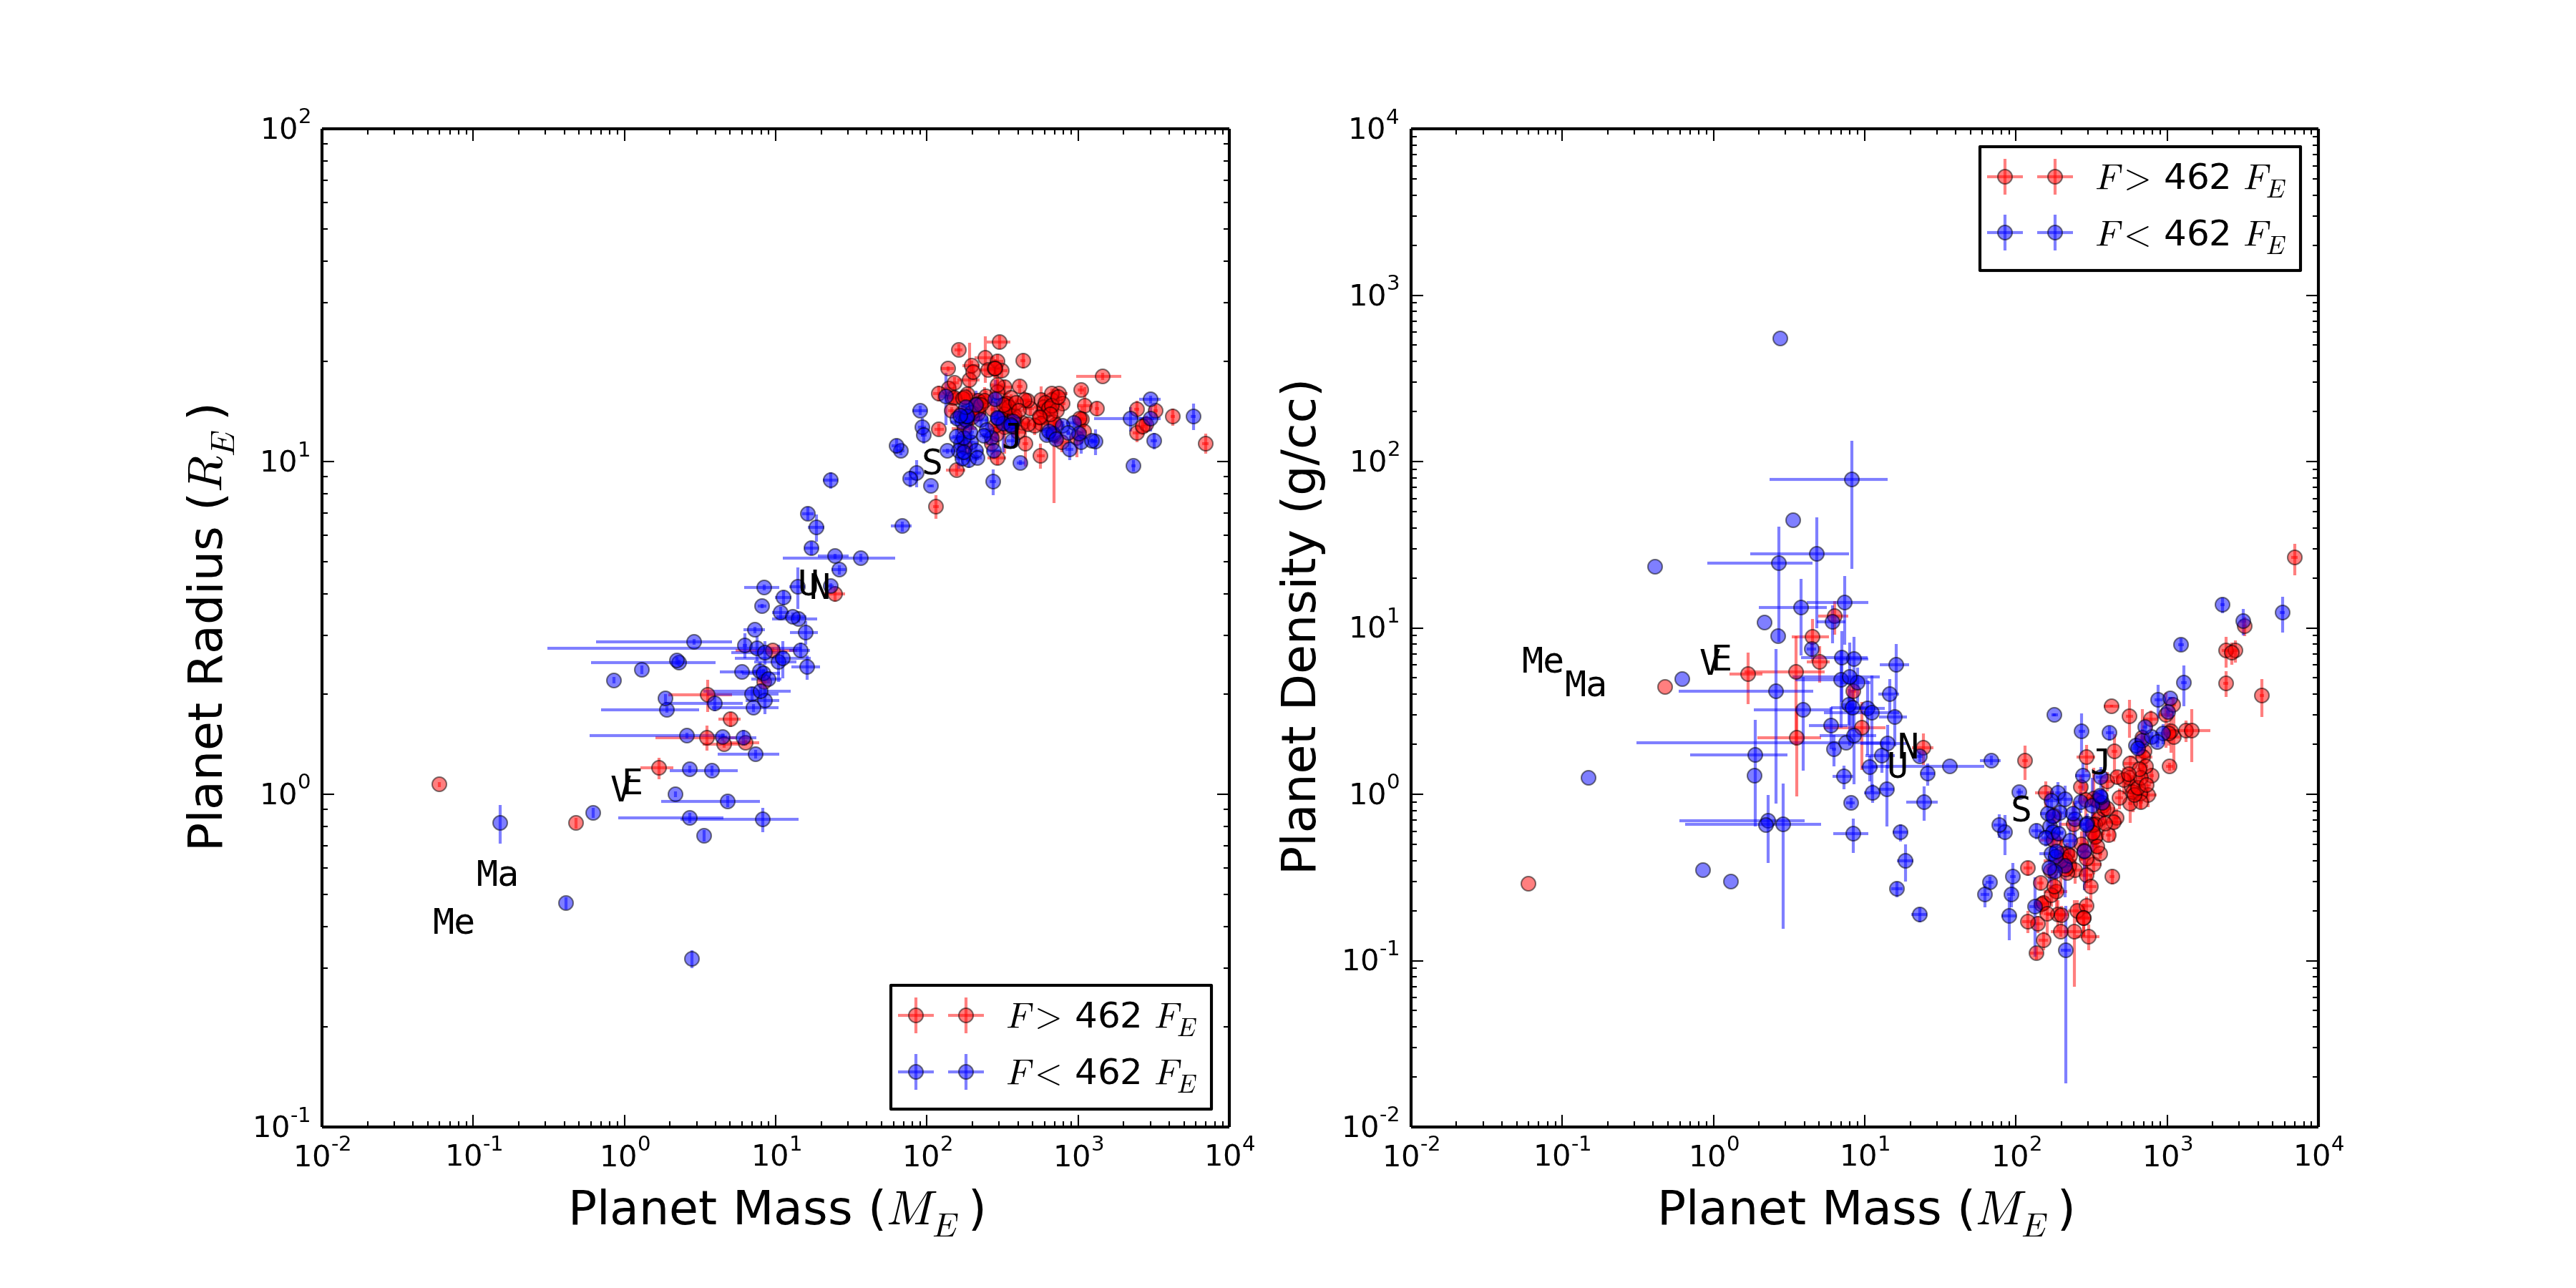
\includegraphics[width=6in]{mrf.png} 
   \caption{\small \textbf{Left:} Radius vs. mass for 243 exoplanets with measured masses and radii.  Below $150 \mearth$, planet radius increases with planet mass; above $150 \mearth$, planet radius slightly decreases with planet mass.  The solar system planets are shown as black triangles for comparison.  Planets receiving lower than the median incident flux in this sample (462 times the incident flux at Earth) are blue; those receiving higher than the median incident flux are red.    For giant planets (above about $150 \mearth$), planet radius increases with increasing incident flux, whereas for the smaller planets, the relation between radius and incident flux is uncertain.  \textbf{Right:} Density vs. mass for 243 exoplanets with measured masses and radii.  The break at $150 \mearth$ separates the low-mass planets, for which density decreases with increasing mass, from the high-mass planets, for which density increases with increasing mass.  The flux coloration is the same as the left figure.}
\label{fig:mrf}
\end{figure*}

\begin{figure*}[htbp] %  figure placement: here, top, bottom, or page
   \centering
    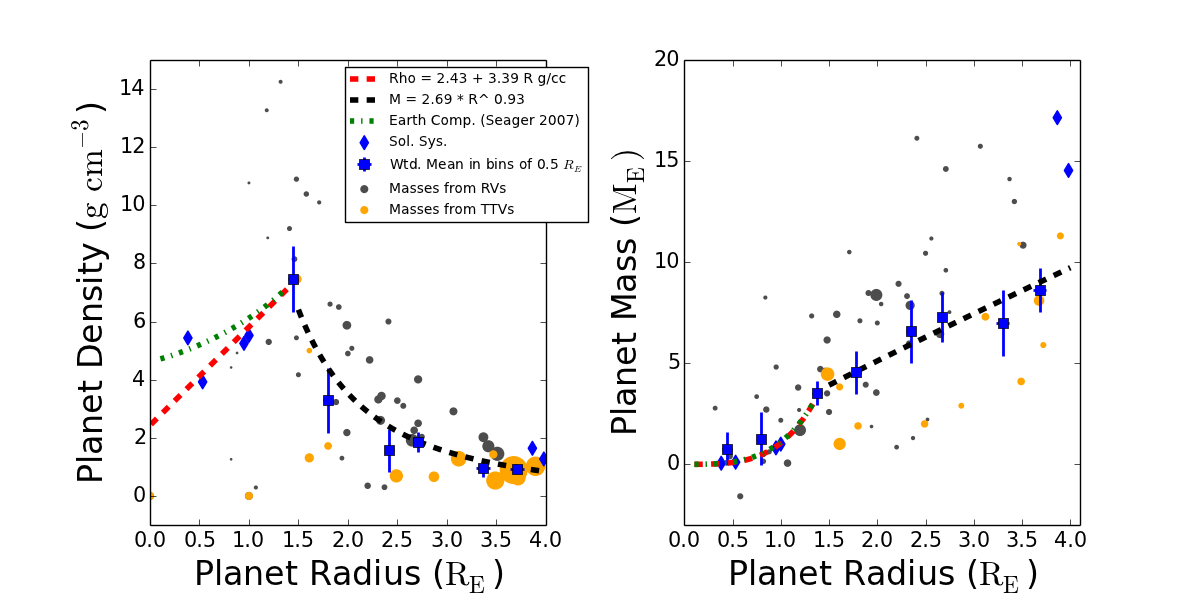
\includegraphics[width=6in]{mr_small.png} 
   \caption{\small \textbf{Left:} Mass vs. radius for 59 exoplanets and 1$\sigma$ error bars (errors were not allowed to go below 10\% of the mass or 5\% of the radius).  The black dashed line is the weighted linear fit given in equation \ref{eqn:mr_relation}.  The blue points are the weighted mean exoplanet mass in bins of $1\rearth$, with error bars representing the uncertainty in the means.  The magenta letters indicate solar system planets.  The weighted means and solar system planets are to guide the eye only; they were not used in calculating the linear fit. \textbf{Right:} Density vs. radius for planets with $\sigma_\rho < 6.5 \gcc$.  Note that no exoplanets smaller than $1\rearth$ have densities determined to better than 6.5 \gcc.  The black dashed line represents the same linear mass-radius relation as left.  The blue points are the weighted mean densities in bins of $1\rearth$.  Earth�s density is shown as the green dotted line.}
   \label{fig:rm_4}
\end{figure*}


\begin{figure*}[htbp] %  figure placement: here, top, bottom, or page
   \centering
    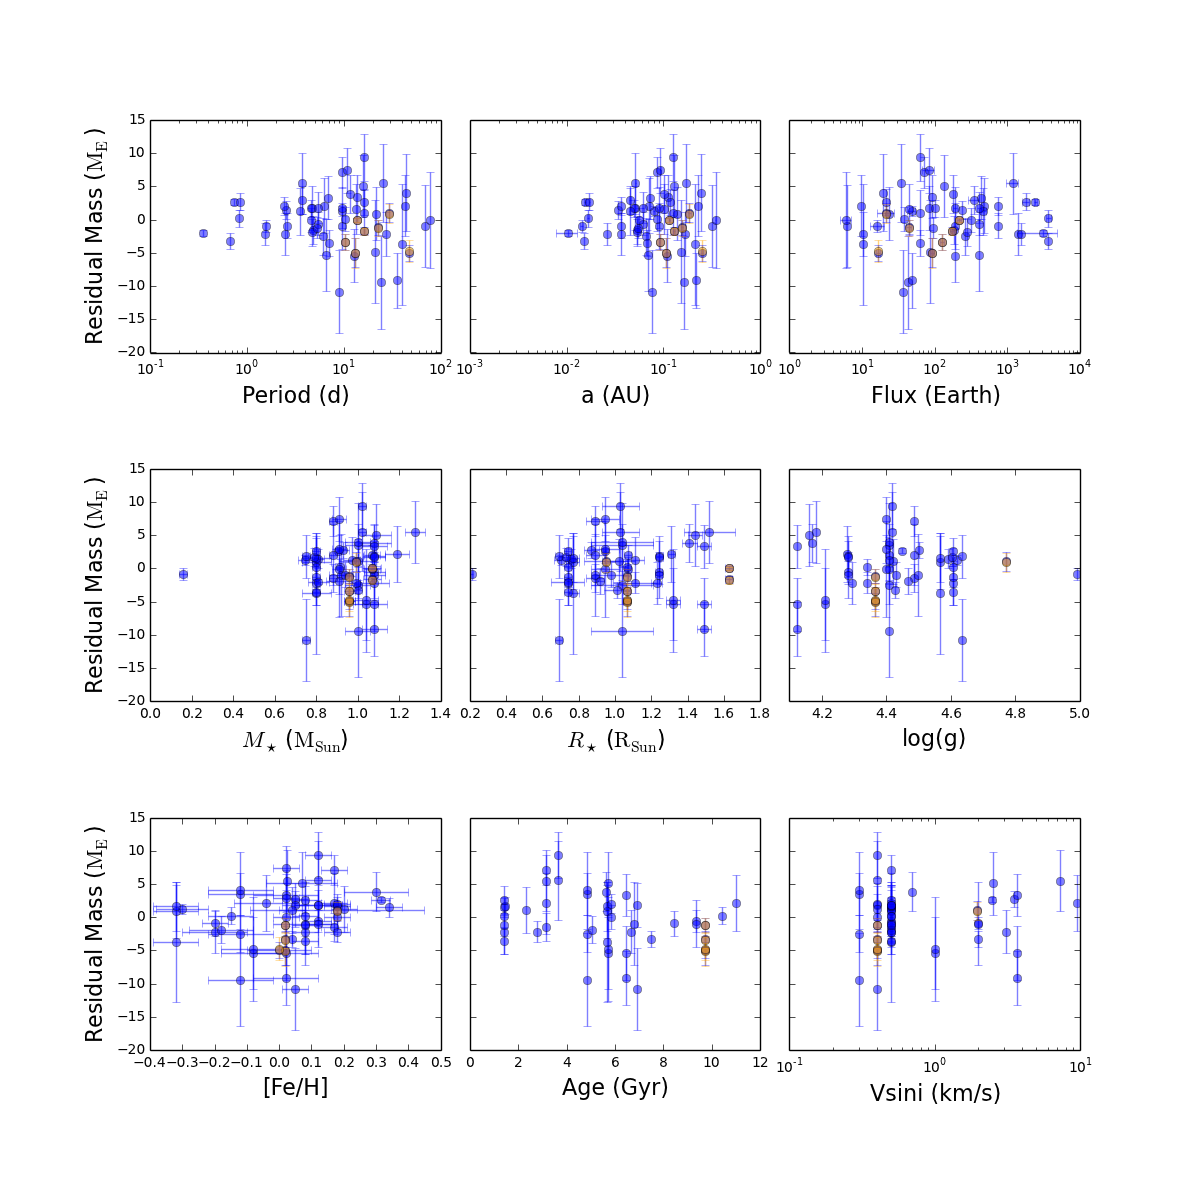
\includegraphics[width=6in]{mr_resids.png} 
   \caption{\small Mass and radius residuals (measured minus predicted mass or radius) versus various orbital and stellar properties for planets with $\rpl  < \rspecial$ and 1$\sigma$ uncertainties.  There is a weak correlation (R=0.25, 2$\sigma$ confidence) between residual mass and stellar metallicity (bottom left); none of the other residuals show correlation.  The spread of the residuals is higher at long orbital periods and orbital distances than at short orbital periods and orbital distances (top row), indicating a possibly larger diversity of exoplanet compositions at large orbital distances than close-in.}
   \label{fig:resids}
\end{figure*}

%%%%%%%%%%%%% Discussion %%%%%%%%%%%%%%%%%%%%%%%%%%%%%%%%
\clearpage

\bibliography{exoplanet_papers}{}
\bibliographystyle{apj}

\end{document}  